\chapter{Introduction}
\section{Electronic Structure for Materials Science}
In 1987 Henry Ehrenreich published an article in Science called
``Electronic Theory for Materials Science". The article begins
with what might now be considered a bold statement:

\begin{quote}
Theoretical Materials Science remains to be invented as a discipline, and for good reason.
\end{quote}

The reason he supplies is that materials processing, historically, was a craft. 

As a striking example of materials science as a craft we consider Roman concrete.
Sometime over two millenia ago Roman engineers learned to manufacture concrete 
from a mixture of volcanic sands called pozzolana,
which take its name from Pozzuoli near Naples, mixed with quicklime, an aggregate, and seawater.
This concrete was of striking quality. The pantheon today remains standing 
built with the same concrete poured centuries before.
This concrete was particularly resistant to degradation in the presence of moisture.
\footnote{For a description of roman concrete and its use at the port at Pouzol see: Mariano Vasi, 
Itineraire Instructif de Rome à Naples, ou, Description Generale des Monumens Anciens et Modernes, 
Rome: [Mariano Vasi]. 1813, de Beer Itb 1815 V.}. 
This concrete was manufactured without any specific knowledge of the microstructure and 
chemistry of the concrete. How it even came to be discovered is somewhat mysterious.

Equally crafty we have mediaeval blacksmith's who learned to manipulate the 
hardness of swords and shields by the alloying of metals and precise control of heat. 
Again the theoretical model they worked with in there heads had no conception of 
the atomic composition of the weapons or the size and character of the metallic grains within them. 

In each case the material practitioner's expertise was not accumulated based on reasoning 
from first principles but based on experience, trial and error, and craft.

A comprehensive atomic theory describing the way atoms bind, the forces acting on them, 
and the techniques to solve these equations has only arisen in the last 100 years. 
Over the past 40 years the combination of the theory and access to computers 
means the possibility of constructing accurate models of materials 
systems beginning from the arrangment of the constituent atoms has
progressed giving rise to the large field of first principles or {\it ab initio} modelling.

The extent to which theoretical materials science as a discipline has evolved over this period of time is worth examining. 
It is important because the character of this evolution dictates which directions of research may prove most
immediately fruitful. It is also important because it allows researchers to identify the avenues
of research that are inefficient, that are potentially obscuring knowledge, and convoluting 
what is already understood. 

To chart this evolution we may begin from Ehrenreich's survey of the field from 30 years ago.

Ehrenreich identified four points that either characterized the state 
of the field of theoretical material science at the time or constituted essential principles 
that a satisfactory theory of materials must uphold:
%
\begin{enumerate}[i)]
\item Theory must be closely linked to experiment.
\item Ab initio calculations without approximations are virtually impossible except in model systems.
\item Approximations are frequently based on prior experience rather than on theoretical justification.
\item The study of trends in the properties of homologous materials 
      is a crucial ingredient of a credible theoretical framework.
\end{enumerate}
%
Based on these four observations provide a useful framework to 
analyze the current state of the field.

\section{The Rise of the Computer}
\label{sec:riseofcomp}
We shall begin, naturally, with the second of Ehrenreich's points, 
which addresses the state of ab initio calculations
and the inherent difficulties in performing them. 

The intervening thirty years has seen an enormous extension of computing capacity. 

To demonstrate this we may contrast the machines available at the time
he was writing to those that are available at the present time of writing (2017). 

In 1987 an example of a state of the art computer would be the Connection Machine.
\footnote{One of the employees at Thinking Machines Corporation,
the company building the connection machine, was Richard Feynman.
For an interesting discussion of the work they
did at Thinking Machines and Feynman's time there see W. Daniel
Hillis' article in Physics Today 42, 2, 78 (1989).
There was a strong focus on design at the company. Some of that
work can be found at Tamiko Thiel's page}%; \url{http://www.tamikothiel.com/theory/cm_txts/di-frames.html}}

The CM-2 was launched in 1987 It was configured with up to 512 MB of RAM and 25 GB of RAID
hard disk space. It had 65K microprocessors (each with 600 bytes of memory). 
%Support for 32 bit floating point operations meant just over 2048 processors in practice per machine.

By contrast the HPC machine presently accessible to the author 
is more easily measured in nodes. Each node in a machine has 2x12 core Intel Broadwell processors.
Each node has 128 GB RAM and 120 GB static storage. The machine has in total 720 nodes. 
The processors themselves have up to 10 cores with clock speeds (roughly the speed the
processor can execute instructions) on the order of 3 GHz a clock speed of 12.5 MHz would be representative in 1987. 
Each processor has abundant cache space of 10x 256 KiB L2 Cache, and 25 MiB of L3 cache 
(compared to 600 bytes in the connection machine). 
There could be on the order of 3 billion transistors in a single microprocessor now;
in 1987 that number would be closer to 100,000. 

Listing specifications doesn't necessarily clarify how much more powerful machines have become, 
but it is striking that in terms of speed, storage, and transistor density there are 3-5 orders of magnitude 
improvements in each category. The stability and optimization of compilers and the ease of programmability
of the machines has also improved.

This constant development of computing capacity has played an important component in enabling
{\it ab initio} calculations. 

\subsection{Scales of Materials Modelling}
What are the scales involved in connecting atomic systems where quantum mechanics is important
to macroscopic systems? Chemists arrived at the mol as a convenient unit for describing
quantities of atoms which is on the order of $10^{23}$ atoms. This is clearly impractical.

More realisitically a suitably macroscopic specimen might be considered to be on the 
order of 200 nm$^{3}$ of material. A sample of material of this size is of the 
same order as the wavelength of visible light and could be
resolved with an optical microscope. Assuming an atomic spacing of 1 tenth of a nanometer 
a dynamical simulation of around 8 billion atoms done using quantum mechanics 
could be considered a quantum mechanical simulation of a macroscopic system. 

To give an idea of the time required to perform a well converged quantum simulation 
250 Fe atoms required 4 hours on 96 nodes of the computer with the same 
specifications noted earlier. There are 2000 electrons in the simulation which must be allowed
to rearrange themselves so they find their energetic minimum. This calculation yields forces on every 
atom that are calculated to an accuracy greater than 0.1 eV/A (electron volts per angstrom).
This accuracy is determined by the limitations of the theory employed to perform the simulation
rather than numerical limitations.

If computer technology continues developing at the same rate it has
over the previous 30 years than within 60 years, with no developements in the numerical techniques, 
quantum mechanical simulations of systems of millions of atoms should be feasible
within a similar amount of computing time. 

If dynamical properties are of interest the atoms motion must be propagated forward. 
If a time step of a femtosecond $(10^{-15}s)$ is taken between evaluations of the 
forces generating a picosecond of data $(10^{-12}s)$ would require about 5 months 
computing time. Another 12 orders of magnitude efficiency would remain to be found to 
simulate the motion of particles on time scales more familiar to everyday experience.

These considerations are artificial for two important reasons. The first
is I strongly suspect computational power will not continue developing at the rate
seen over the previous 30 years. 

The second is that even if computational resources did continue growing 
at an equivalent rate; simulations of the nature might be of little value.
The objective of {\it ab initio} modeling is to extract meaningful information
about trends and characteristic properties of different classes of materials. 
Massive simulations generate such a quantity of data they may obscure 
reasoning and consume resources without providing insight and general principles.

If studying trends in homologous materials is truly a necessary component of a satisfactory
theory then these simulations would have to be repeated over and over again.
Furthermore macroscopic materials mechanics does not require a quantum description.
Thermodynamics and continuum mechanics provides a suitable description of the physics of these systems. 

The development in computing hardware is in some ways the easy part to chart. 
Clock speeds, transistor density, and the proliferation of high 
performance computing clusters with fast interconnects have greatly extended 
the range of problems that can be treated with numerical simulations
simply by providing more horse power.

Along with advances in hardware there has been contemporaneous methodological developments.
These include compiler optimization, development of modern programming languages, 
shared libraries, object orientation, and stable open source platforms for 
code development, testing, and sharing. All of which can be binned in the 
category computers and computing culture.

The important theoretical advances, i.e., the physical principles and
mathematical techniques that enable material's science are more difficult to quantify. 
Difficult to quantify in what exactly they are and what they have enabled. In the
next section we try and identify the major pillars of materials modelling.

\section{Computational Craft}
%Given a really good computer what would you like to do with it?
%Write documents and send them to people? Create a system where the computers share files
%with each other? Listen to music? Watch films? Learn Things? Compute things? The latter is in some
%ways becoming a niche application of computers.

What sort of things should a computer compute? A theoretical material scientist
can answer this question definitively. One would like to:
"... compute groundstate properties such as cohesive energies, interatomic forces, 
charge transfer, and magnetic moments, and also excitation spectra described 
by the one-electron Green's function."\cite{anderson75} 

The theoretical engines driving progress in numerical simulations of materials systems are
largely based on density functional theory, effective separation and treatment of the problem
of treating core-valence electronic interactions, and the various numerical algorithms for 
computing the eigenstates of electrons in material systems, and solving the coupled systems of linear equations which arise 
again and again when doing self-consistent electronic structure calculations.

Looking at the citation metrics, foundational papers in theoretical materials science
number their citations in the tens of thousands. Table~\ref{tab:foundation} lists some of the papers in the field which, as
their citation count suggests, have enabled subsequent research. These techniques fall into
three categories, they are either theoretical justification for a calculation scheme, the description of
a technique that allows for more expedient and/or accurate calculations to be performed, 
or parameterizations of the exchange-correlation functional.

\begin{table}
\resizebox{\columnwidth}{!}{%
\begin{tabular}{|p{6cm}|l|p{6cm}|p{4cm}|}
\hline
Paper & Citations & Development & Category\\
\hline
Inhomogeneous Electron Gas \cite{hohenberg64} & 20,527 & Ground state energy of electron gas is universal functional of the density. & Theory \\
Self-Consistent Equations Including Exchange and Correlation Effects & 26,273 & Self-consistent set of equations for varying electron density. & Theory \\
Linear methods in band theory \cite{andersen75}& 4,822 & Describes LAPW and LMTO approach to electronic structure calculations. & Theory/Implementation \\
Norm-Conserving Pseudopotentials \cite{hamann79} & 2,156 & Nodeless eigenfunctions that match atomic eigenvalues.  & Pseudopotentials \\
Soft self-consistent pseudopotentials in a generalized eigenvalue formalism \cite{vanderbilt90} & 11,560 & Effective pseudopotentials for first row and transition-metal systems  & Pseudopotentials \\
Projector augmented-wave method \cite{blochl94paw} & 19,194 & Generalizes pseudopotential and LAPW methods; allows reconstruction of wavefunctions at nucleus.  & Pseudopotentials \\
Efficacious Form for Model Pseudopotentials \cite{kleinman82} & 3,709 & Reduces number of integrals which need to be calculated & Pseudopotentials \\
Special points for Brillouin-zone integrations \cite{monkhorst76} & 21,361 & Brillouin zone integration & Numerical Integration \\
Ground State of the Electron Gas by a Stochastic Method \cite{ceperley80} & 8,855 & Calculation of the exchange-correlation energy of an electron gas. & Exchange Correlation \\
Self-interaction correction to density-functional approximations for many-electron systems \cite{perdew81} & 11,629 & Parameterization of Ceperley-Alder & Exchange Correlation \\
Accurate and simple analytic representation of the electron-gas correlation energy \cite{perdew91} & 12,296 & Parameterization of exchange correlation functional & Exchange Correlation \\
Atoms, molecules, solids, and surfaces: Applications of the generalized gradient approximation for exchange and correlation \cite{perdew92} & 11,418 & Generalized gradient expansion& Exchange Correlation \\
New Method for Calculating the One-Particle Green's Function with Application to the Electron-Gas Problem & 2,599 & A calculation scheme for
obtaining progressively more accurate approximations to the one-electron Green's function \cite{hedin65} & Theory\\
Electron correlation in semiconductors and insulators: Band gaps and quasiparticle energies \cite{hybertsen86} & 1,929 & Extension of electronic structure calculations to excited states& Theory/Implementation \\
Unified Approach for Molecular Dynamics and Density-Functional Theory \cite{car85} & 5,940 & Combined molecular dynamics and density functional theory & Theory/Implementation \\
High-precision sampling for Brillouin-zone integration in metals \cite{methfessel89} & 2,908 & Brillouin zone integration & Numerical Integration Technique \\
Improved tetrahedron method for Brillouin-zone integrations \cite{blochl94} &  2,986 & Brillouin zone integration & Numerical Integration Technique\\
A new mixing of Hartree–Fock and local density‐functional theories \cite{becke93} & 7,143 & Combining Hartree-Fock and DFT & Exchange Correlation \\
Generalized Gradient Approximation Made Simple \cite{perdew96} & 47,029 & GGA functionals improved.& Exchange Correlation \\
\end{tabular}
}
\caption{Citations are relevant up to Nov. 2017. Citations are according to the journals in which they appear, the actual number of
citations are much higher. These selections have been chosen as representative of the important theoretical and algorithmic developments
which have enabled subsequent research. In some cases there are a number of contemporary papers which
treat the same problems but failed to "catch on" or describe techniques which differ in an incremental way to the works cited here. 
\label{tab:foundation}}
\end{table}

This table is biased towards a "plane wave" conception of electronic structure. 
These methods are suitable for crystalline systems with periodicity and can be pushed 
to describe more disordered systems on the order, as discussed in Sec.\ref{sec:riseofcomp}, of 1000 atoms.. 

To broadly categorize the workers we can say a material scientist 
is interested in crystals, alloys, ceramics, glasses, and possibly elastic materials. They
worry about energy differences on the order of 100 meV. Chemists are interested in molecules, 
tend to use localized basis sets and exploit Monte Carlo methods to obtain energy 
bounds on the order of a few meV. Physicists are interested in lasers and hubbard models and the 
general positions of resonances and asymptotes in very cold materials and wont be discussed further.

If we look at the work done based on parameterization of the exchange correlation functional 
we see the number of citations approaches 100,000. Naturally that figure includes significant 
double counting of citing work but we have also not included cross citations between journals in many of the 
figures quoted so the number is probably representative. This parameterization is based on 
what I consider a highly abstract question. "What might happen if we start squeezing electrons into an imaginary box?".

This imaginary box has been pondered for close to a century now. The practical utility of these considerations is unreasonable. 
The outcome of these considerations have resulted in a family of unremarkable curves that describe some energy relationship between
the number density of electrons at a point in space and an energy. The practical consequence is this curve enables the
structural, electronic, and vibrational properties of an enormous class of materials to be calculated with highly creditable accuracy.

How creditable this approach is returns again to point three. The theoretical justifications for the success of the approach are
secondary to the fact that prior experience suggests these techniques work, and the rate of their acceptance and adoption
seems to have tracked their usage in a positive feedback loop. 
%For instance an article from 12 years ago 

%If you remain unconvinced of the accuracy of the method one can at least acknowledge the social benefit. 
%The sheer number of hours people have been engaged in this harmless occupation, dreaming of 
%electrons in an imaginary box, means they have a hobby that keeps them off the streets and out of trouble.

%The computational price paid to obtain these quantities should be considered. If the amount of numerical
%work required to compute the quantities is excessive it becomes difficult to discuss trends in homologous series of materials, perform
%necessary thermal averages to describe distributions, and even in some cases reproduce exactly the calculation.

\section{Point 3: Justification by Utility}
The observation that materials processing has evolved in the manner of a craft appears to have
been imitated in the development of the theory of materials science.

If you look through a typical electronic structure code it is interesting to look at the routine
responsible for calculating the local exchange correlation potential. The input required is the 
electronic density at a point in space and possibly the gradient of the density at a point. This 
density is inserted as the sole argument in a subroutine and a single number is returned. The curve
returned has little more structure than that given in Fig.~\ref{fig:ldapz}. 
%
\begin{figure}
\begin{center}
\graphicspath{{./intro/}}% GNUPLOT: LaTeX picture with Postscript
\begingroup
  \makeatletter
  \providecommand\color[2][]{%
    \GenericError{(gnuplot) \space\space\space\@spaces}{%
      Package color not loaded in conjunction with
      terminal option `colourtext'%
    }{See the gnuplot documentation for explanation.%
    }{Either use 'blacktext' in gnuplot or load the package
      color.sty in LaTeX.}%
    \renewcommand\color[2][]{}%
  }%
  \providecommand\includegraphics[2][]{%
    \GenericError{(gnuplot) \space\space\space\@spaces}{%
      Package graphicx or graphics not loaded%
    }{See the gnuplot documentation for explanation.%
    }{The gnuplot epslatex terminal needs graphicx.sty or graphics.sty.}%
    \renewcommand\includegraphics[2][]{}%
  }%
  \providecommand\rotatebox[2]{#2}%
  \@ifundefined{ifGPcolor}{%
    \newif\ifGPcolor
    \GPcolortrue
  }{}%
  \@ifundefined{ifGPblacktext}{%
    \newif\ifGPblacktext
    \GPblacktextfalse
  }{}%
  % define a \g@addto@macro without @ in the name:
  \let\gplgaddtomacro\g@addto@macro
  % define empty templates for all commands taking text:
  \gdef\gplbacktext{}%
  \gdef\gplfronttext{}%
  \makeatother
  \ifGPblacktext
    % no textcolor at all
    \def\colorrgb#1{}%
    \def\colorgray#1{}%
  \else
    % gray or color?
    \ifGPcolor
      \def\colorrgb#1{\color[rgb]{#1}}%
      \def\colorgray#1{\color[gray]{#1}}%
      \expandafter\def\csname LTw\endcsname{\color{white}}%
      \expandafter\def\csname LTb\endcsname{\color{black}}%
      \expandafter\def\csname LTa\endcsname{\color{black}}%
      \expandafter\def\csname LT0\endcsname{\color[rgb]{1,0,0}}%
      \expandafter\def\csname LT1\endcsname{\color[rgb]{0,1,0}}%
      \expandafter\def\csname LT2\endcsname{\color[rgb]{0,0,1}}%
      \expandafter\def\csname LT3\endcsname{\color[rgb]{1,0,1}}%
      \expandafter\def\csname LT4\endcsname{\color[rgb]{0,1,1}}%
      \expandafter\def\csname LT5\endcsname{\color[rgb]{1,1,0}}%
      \expandafter\def\csname LT6\endcsname{\color[rgb]{0,0,0}}%
      \expandafter\def\csname LT7\endcsname{\color[rgb]{1,0.3,0}}%
      \expandafter\def\csname LT8\endcsname{\color[rgb]{0.5,0.5,0.5}}%
    \else
      % gray
      \def\colorrgb#1{\color{black}}%
      \def\colorgray#1{\color[gray]{#1}}%
      \expandafter\def\csname LTw\endcsname{\color{white}}%
      \expandafter\def\csname LTb\endcsname{\color{black}}%
      \expandafter\def\csname LTa\endcsname{\color{black}}%
      \expandafter\def\csname LT0\endcsname{\color{black}}%
      \expandafter\def\csname LT1\endcsname{\color{black}}%
      \expandafter\def\csname LT2\endcsname{\color{black}}%
      \expandafter\def\csname LT3\endcsname{\color{black}}%
      \expandafter\def\csname LT4\endcsname{\color{black}}%
      \expandafter\def\csname LT5\endcsname{\color{black}}%
      \expandafter\def\csname LT6\endcsname{\color{black}}%
      \expandafter\def\csname LT7\endcsname{\color{black}}%
      \expandafter\def\csname LT8\endcsname{\color{black}}%
    \fi
  \fi
    \setlength{\unitlength}{0.0500bp}%
    \ifx\gptboxheight\undefined%
      \newlength{\gptboxheight}%
      \newlength{\gptboxwidth}%
      \newsavebox{\gptboxtext}%
    \fi%
    \setlength{\fboxrule}{0.5pt}%
    \setlength{\fboxsep}{1pt}%
\begin{picture}(5760.00,3960.00)%
    \gplgaddtomacro\gplbacktext{%
      \csname LTb\endcsname%%
      \put(1078,2420){\makebox(0,0)[r]{\strut{}$-0.1$}}%
      \put(1078,2684){\makebox(0,0)[r]{\strut{}$-0.08$}}%
      \put(1078,2948){\makebox(0,0)[r]{\strut{}$-0.06$}}%
      \put(1078,3211){\makebox(0,0)[r]{\strut{}$-0.04$}}%
      \put(1078,3475){\makebox(0,0)[r]{\strut{}$-0.02$}}%
      \put(1078,3739){\makebox(0,0)[r]{\strut{}$0$}}%
      \put(1210,2200){\makebox(0,0){\strut{}$0$}}%
      \put(2041,2200){\makebox(0,0){\strut{}$0.2$}}%
      \put(2871,2200){\makebox(0,0){\strut{}$0.4$}}%
      \put(3702,2200){\makebox(0,0){\strut{}$0.6$}}%
      \put(4532,2200){\makebox(0,0){\strut{}$0.8$}}%
      \put(5363,2200){\makebox(0,0){\strut{}$1$}}%
    }%
    \gplgaddtomacro\gplfronttext{%
      \csname LTb\endcsname%%
      \put(198,3079){\rotatebox{-270}{\makebox(0,0){\strut{}Energy (Ry.)}}}%
      \csname LTb\endcsname%%
      \put(4376,3566){\makebox(0,0)[r]{\strut{}PZ Correlation Energy}}%
    }%
    \gplgaddtomacro\gplbacktext{%
      \csname LTb\endcsname%%
      \put(946,704){\makebox(0,0)[r]{\strut{}$-1$}}%
      \put(946,915){\makebox(0,0)[r]{\strut{}$-0.8$}}%
      \put(946,1126){\makebox(0,0)[r]{\strut{}$-0.6$}}%
      \put(946,1338){\makebox(0,0)[r]{\strut{}$-0.4$}}%
      \put(946,1549){\makebox(0,0)[r]{\strut{}$-0.2$}}%
      \put(946,1760){\makebox(0,0)[r]{\strut{}$0$}}%
      \put(1078,484){\makebox(0,0){\strut{}$0$}}%
      \put(1935,484){\makebox(0,0){\strut{}$0.2$}}%
      \put(2792,484){\makebox(0,0){\strut{}$0.4$}}%
      \put(3649,484){\makebox(0,0){\strut{}$0.6$}}%
      \put(4506,484){\makebox(0,0){\strut{}$0.8$}}%
      \put(5363,484){\makebox(0,0){\strut{}$1$}}%
    }%
    \gplgaddtomacro\gplfronttext{%
      \csname LTb\endcsname%%
      \put(198,1232){\rotatebox{-270}{\makebox(0,0){\strut{}Energy (Ry.)}}}%
      \put(3220,154){\makebox(0,0){\strut{}$\rho$ (e/a.u.$^{3}$)}}%
      \csname LTb\endcsname%%
      \put(4376,1587){\makebox(0,0)[r]{\strut{}PZ Exchange Energy}}%
    }%
    \gplbacktext
    \put(0,0){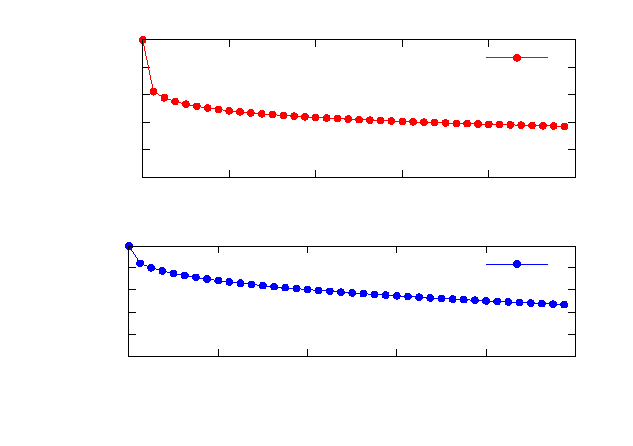
\includegraphics{pz}}%
    \gplfronttext
  \end{picture}%
\endgroup

\caption{Perdew-Zunger parameterization of the correlation and exchange energies for an electron gas.
This curve and those like it enable a great deal of contemporary materials modelling. For reference
a crystal of iron would have an electronic density of around 0.36 e/a.u.$^{3}$ (electrons per cubic
atomic unit). A silicon crystal would have an electronic density in the range of 0.02 e/a.u.$^{3}$,
carbon in the diamond conformation would be around 0.1 e/a.u.$^{-3}$.  
\label{fig:ldapz}.}
\end{center}
\end{figure}
%
Curves of this type have been used to perform calculations and simulations for 
materials composed of elements from across the periodic table. They have been
used to compute all the properties of interest, cohesive energies, magnetic moments,
etc. with varying degrees of success.

Yet in all manner of crystalline systems this functional enables the theoretical
prediction of very accurate ground state properties and structures. 

Another successful theoretical development is pseudopotentials. Focusing on the valence electrons 
has worked for chemistry.

\section{Bayesian Materials Science}
The ubiquity of access to {\it ab initio} data has had a significant impact on 
Ehrenreich's first point: experimental corroboration. 
Cursory surveys of the literature demonstrate the increasing frequency of 
appearance of publications which contain no original experimental work. 

This is partly down to the high level of specialization of contemporary 
researchers and research groups. Previously, the distinction between
an experimental materials scientist and a theoretical one was not so dramatic. 
In addition many important theoretical developments came 
from the context of attempting to explain a new set of experimental data.
%This paragraph needs research:
%Bethe's calculation of the hyperfine? shift, the recursion work on the magnetic 
%moment of $FeAl_{3}$, I think Bardeen mentioned his work on superconductivity was
%initiated when they were trying, Shockley's work on the transistor. (A good source 
%for these sorts of anecdotal history can be found in Nobel prize banquet speeches.)
Ehrenreich's four points help clarify a desirable objective for materials modelling:
a minimal theoretical model informed by {\it ab initio} calculations that accounts for 
experimental data, and {\emph predicts} quantitatively trends in material properties. 

In these notes the possibility of exploiting the invariance theorem 
and recursion techniques is assessed as the optimal framework
for achieving this. 

A metric for the quality of the approach can be defined using 
Bayesian probability theory. The Bayesian framework lets us define a metric 
that increases as the number of free parameters in the model is reduced,
and the reproduction of target experimental data is increased, 
with a bound on optimal predictions.

The posterior on the parameters of the model can be assessed:
%
\begin{equation}
\label{eq:bayes}
P(\mathbf{w}|D, \mathcal{H}_{i}) = 
\frac{P(D|\mathbf{w}, \mathcal{H}_{i})P(\mathbf{w}|\mathcal{H})}{P(D|\mathcal{H}_{i})},
\end{equation}
%
where D, the target data, can constitute a combination of {\it ab initio} and experimental data. 
Eq.~\ref{eq:bayes} McKay summarises as:
%
\begin{equation}
{\rm Posterior} = \frac{{\rm Likelihood} \times {\rm Prior}}{{\rm Evidence}}
\end{equation}
%
\begin{equation}
\label{eq:bayesH}
P(\mathcal{H}_{i}|D) \propto P(D|\mathcal{H}_{i})P(\mathcal{H}_{i})
\end{equation}
%
\begin{equation}
\label{eq:bayesH}
P(D|\mathcal{H}_{i}) = P(D|\mathbf{w}, \mathcal{H}_{i})P(\mathbf{w}|\mathcal{H}_{i})d\mathbf{w}
\end{equation}
%
Models (hypotheses) of material systems can then be ranked according to Eq.~\ref{eq:bayesH}.

\section{Prospective}
The purpose of these notes are to establish a comprehensive framework 
for incorporating knowledge about material systems into models that can be rapidly
instantiated.

The general procedure is to use ab initio data to map 
to rigorous local models of the atomic environment. The local models
of atomic interaction become easier to store, physical intuition is clarified
and the knowledge obtained becomes persistent. Finally the quality of the models
can be quantified and improved systematically with reference to experiment using
inference techniques.

Subsequent chapters will discuss the theory underlying each of these planks; a
theory of the local atomic environment, a theory of electronic excitations, long
range order in material systems, and bayesian techniques. All of these techniques
have been developed by other workers over a number of years but collecting 
them into a single place still seems a worthwhile endeavour.

In chapter \ref{chap:odlr} the passage from discrete atomic models to continuum mechanics
where collective variables, for instance stress and strain tensors, arise is discussed. 
In Chapter \ref{chap:bayes} the criterion for assessing the quality of {\it ab initio} 
models is discussed which ranks models positively according to their ability to 
describe target experimental data and penalizes them for the number of 
adjustable parameters that enter their description.

While the quantum paradigm is well establish the amount of normal science it motivates
essentially charting and calculating the properties of normal matter means there is 
an indeterminate scope for puzzle solving. The process of setting up and solving Schr\"odingers
equation over and over for increasingly complex systems would seem tedious if it weren't so enjoyable.


